% --------------------------------------------------------------
%                           Set Up
% --------------------------------------------------------------
 
\documentclass[12pt]{article}
 
\usepackage[margin=1in]{geometry} 
\usepackage{amsmath,amsthm,amssymb}
\usepackage{listings}
\usepackage{xcolor}
\usepackage{graphicx}
\usepackage{subcaption}
\usepackage{listings}
\usepackage{xcolor}
\usepackage{comment}
\usepackage{hepnames}
\usepackage{longtable}
 
\definecolor{codegreen}{rgb}{0,0.6,0}
\definecolor{codegray}{rgb}{0.5,0.5,0.5}
\definecolor{codepurple}{rgb}{0.58,0,0.82}
\definecolor{backcolour}{rgb}{0.95,0.95,0.92}
 
\lstdefinestyle{mystyle}{
    backgroundcolor=\color{backcolour},   
    commentstyle=\color{codegreen},
    keywordstyle=\color{magenta},
    numberstyle=\tiny\color{codegray},
    stringstyle=\color{codepurple},
    basicstyle=\ttfamily\footnotesize,
    breakatwhitespace=false,         
    breaklines=true,                 
    captionpos=b,                    
    keepspaces=true,                 
    numbers=left,                    
    numbersep=5pt,                  
    showspaces=false,                
    showstringspaces=false,
    showtabs=false,                  
    tabsize=2
}
 
\lstset{style=mystyle}
 
\definecolor{codegreen}{rgb}{0,0.6,0}
\definecolor{codegray}{rgb}{0.5,0.5,0.5}
\definecolor{codepurple}{rgb}{0.58,0,0.82}
\definecolor{backcolour}{rgb}{0.95,0.95,0.92}
\definecolor{deepblue}{rgb}{0,0,0.5}
\definecolor{deepred}{rgb}{0.6,0,0}
\definecolor{deepgreen}{rgb}{0,0.5,0}
 
\lstdefinestyle{mystyle}{
    backgroundcolor=\color{backcolour},   
    commentstyle=\color{codegreen},
    keywordstyle=\color{deepred},
    numberstyle=\tiny\color{codegray},
    stringstyle=\color{deepblue},
    basicstyle=\ttfamily\footnotesize,
    breakatwhitespace=false,         
    breaklines=true,                 
    captionpos=b,                    
    keepspaces=true,                 
    numbers=left,                    
    numbersep=5pt,                  
    showspaces=false,                
    showstringspaces=false,
    showtabs=false,                  
    tabsize=2
}
 
\lstset{style=mystyle}
 
\newcommand{\N}{\mathbb{N}}
\newcommand{\Z}{\mathbb{Z}}
 
\newenvironment{theorem}[2][Theorem]{\begin{trivlist}
\item[\hskip \labelsep {\bfseries #1}\hskip \labelsep {\bfseries #2.}]}{\end{trivlist}}
\newenvironment{lemma}[2][Lemma]{\begin{trivlist}
\item[\hskip \labelsep {\bfseries #1}\hskip \labelsep {\bfseries #2.}]}{\end{trivlist}}
\newenvironment{exercise}[2][Exercise]{\begin{trivlist}
\item[\hskip \labelsep {\bfseries #1}\hskip \labelsep {\bfseries #2.}]}{\end{trivlist}}
\newenvironment{problem}[2][Problem]{\begin{trivlist}
\item[\hskip \labelsep {\bfseries #1}\hskip \labelsep {\bfseries #2.}]}{\end{trivlist}}
\newenvironment{question}[2][Question]{\begin{trivlist}
\item[\hskip \labelsep {\bfseries #1}\hskip \labelsep {\bfseries #2.}]}{\end{trivlist}}
\newenvironment{corollary}[2][Corollary]{\begin{trivlist}
\item[\hskip \labelsep {\bfseries #1}\hskip \labelsep {\bfseries #2.}]}{\end{trivlist}}

\newenvironment{solution}{\begin{proof}[Solution]}{\end{proof}}

\setlength\parindent{0pt}
 
\begin{document}
 
% -------------------------------------------------------------- 
%                         Start here
% --------------------------------------------------------------
 
\title{Homework }
\author{Timothy Holmes\\ %replace with your name
PHY 442 Computational Physics}

\maketitle

\section*{Problem 1}

The ordinary differential equation is gave by

$$
\frac{dy}{dt} = e^{t}sin(y).
$$

This ODE has the separable solution of

$$
y(t) = 2cot^{-1}(exp(c_{1} - e^{t})).
$$

To better understand what the different numerical methods are plotting it is beneficial to solve for the analytical method first. Comparing the known analytical solution will tell a lot about the numerical solution. Plotting the analytical solution can be found by using some Matlab code such as

\begin{lstlisting}[language=Matlab, caption= ]
figure(1)
hold on
t = 0:0.01:10;
c = exp(-exp(t))*cot(3/2);
y = 2*acot(exp(c - exp(t)));

plot(t, y)
\end{lstlisting}

which produces the what can be seen in Figure 1. One major thing to note is that each of these methods will have an initial $y$ value of $y_{0} = 3$. Therefore, all of our numerical plots will have the line starting at $t = 0$ and $y = 3$. But it is clear to see that this function converges just after $y = 3$. In fact this function converges to $y = 3.142$, meaning that if a numerical method  picks a point over the line $y = 3.142$ the method will already off. There is a lot of information to unpack from Figures 2 and 3. Figure 2 shows all of the numerical methods each with 4 various step sizes and plotted with $t = 5$. While Figure 3 isn't much different, Figure 3 shows all of the numerical methods each with 4 various step sizes and plotted with $t = 10$. With out looking into any of the details and only looking at the raw images, it is clear that the only numerical method that was successful was the Runge-Kutta 45 Adaptive Method. The other 3 numerical methods all had numerical errors. Increasing the time to $t = 10$ only intensified the error. Once the first calculation error occurs the algorithm continues to build off that error bringing the solution further away from the correct results. Changing the step sizes does limit how bad this error gets as we should expect. The step sizes are too large for this ODE, remember, the $y_{0} = 3$ and the function converges shortly after this value. 



\begin{figure}[h!]
    \centering
    {{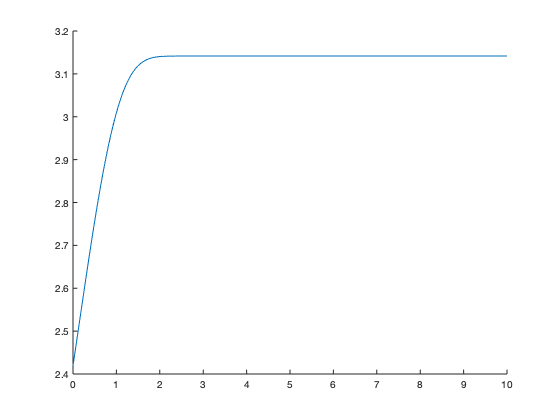
\includegraphics[width=15cm]{problem_1_analytical_sol.png}}}%
    \qquad
    \caption{Analytical solution for the problem 1 ODE.}%
    \label{fig:example}%
\end{figure}


\begin{figure}[htp]
\centering

\begin{subfigure}{0.49\columnwidth}
\centering
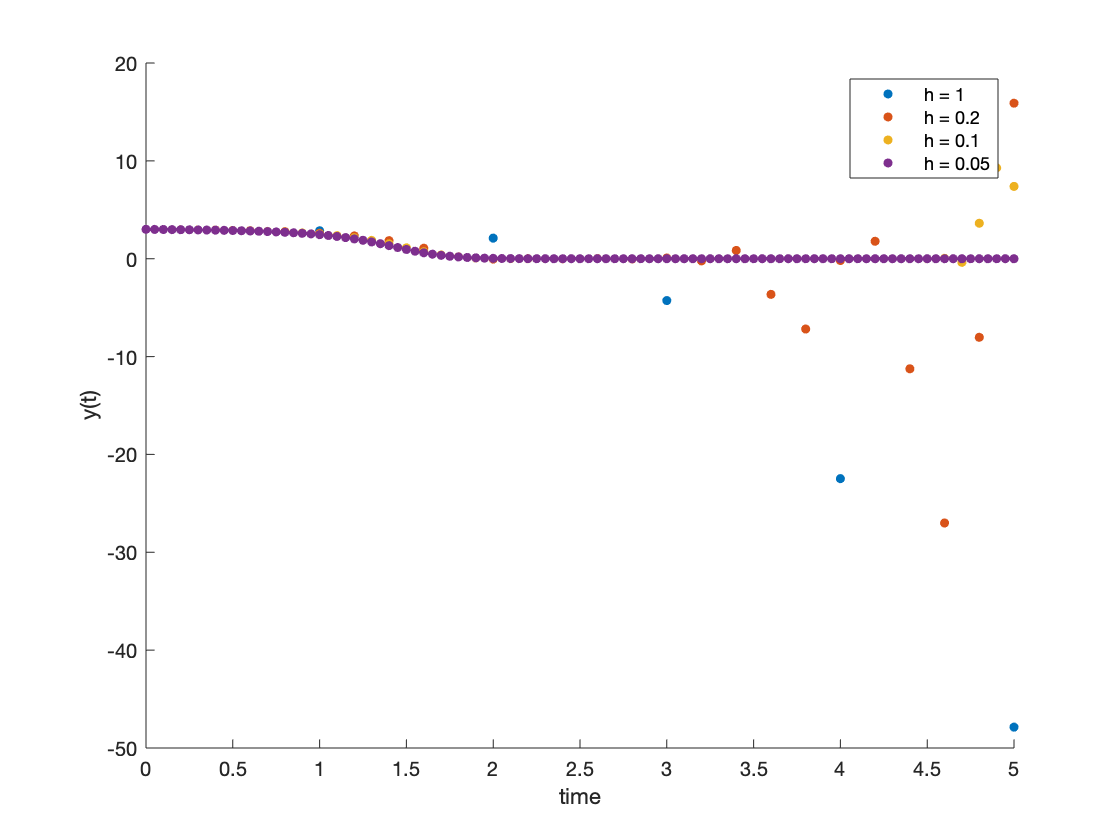
\includegraphics[width=\textwidth]{euler_t_5.png}
\caption{Euler Method}
\label{fig:time1}
\end{subfigure}\hfill
\begin{subfigure}{0.49\columnwidth}
\centering
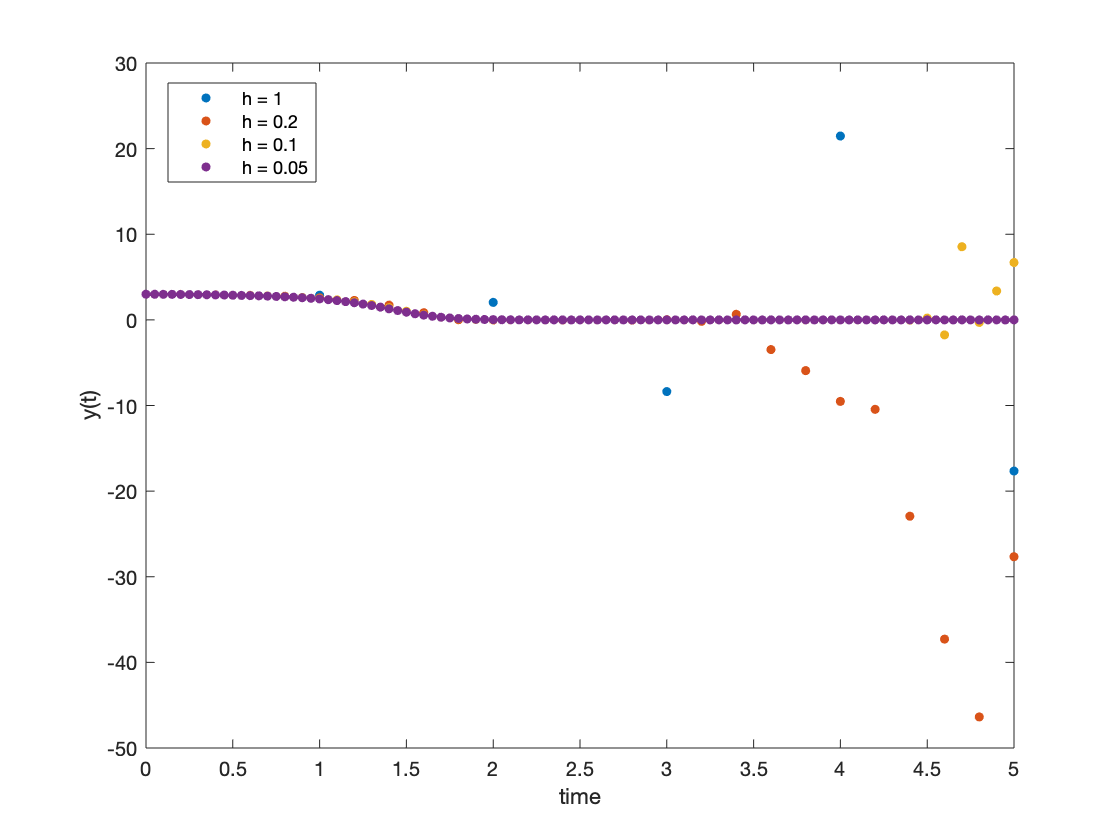
\includegraphics[width=\textwidth]{euler_mid_t_5.png}
\caption{Euler Midpoint Method}
\label{fig:time2}
\end{subfigure}

\medskip

\begin{subfigure}{0.49\columnwidth}
\centering
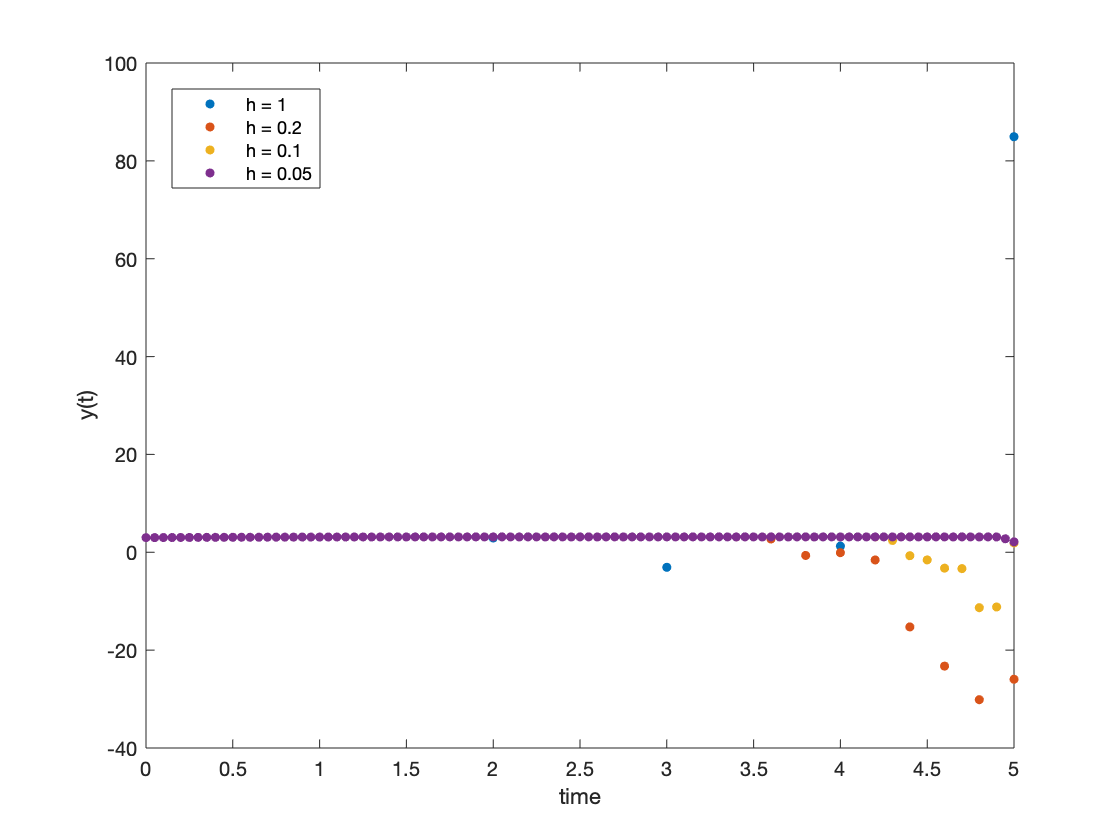
\includegraphics[width=\textwidth]{rk_t_5.png}
\caption{Runge-Kutta Method}
\label{fig:time3}
\end{subfigure}\hfill
\begin{subfigure}{0.49\columnwidth}
\centering
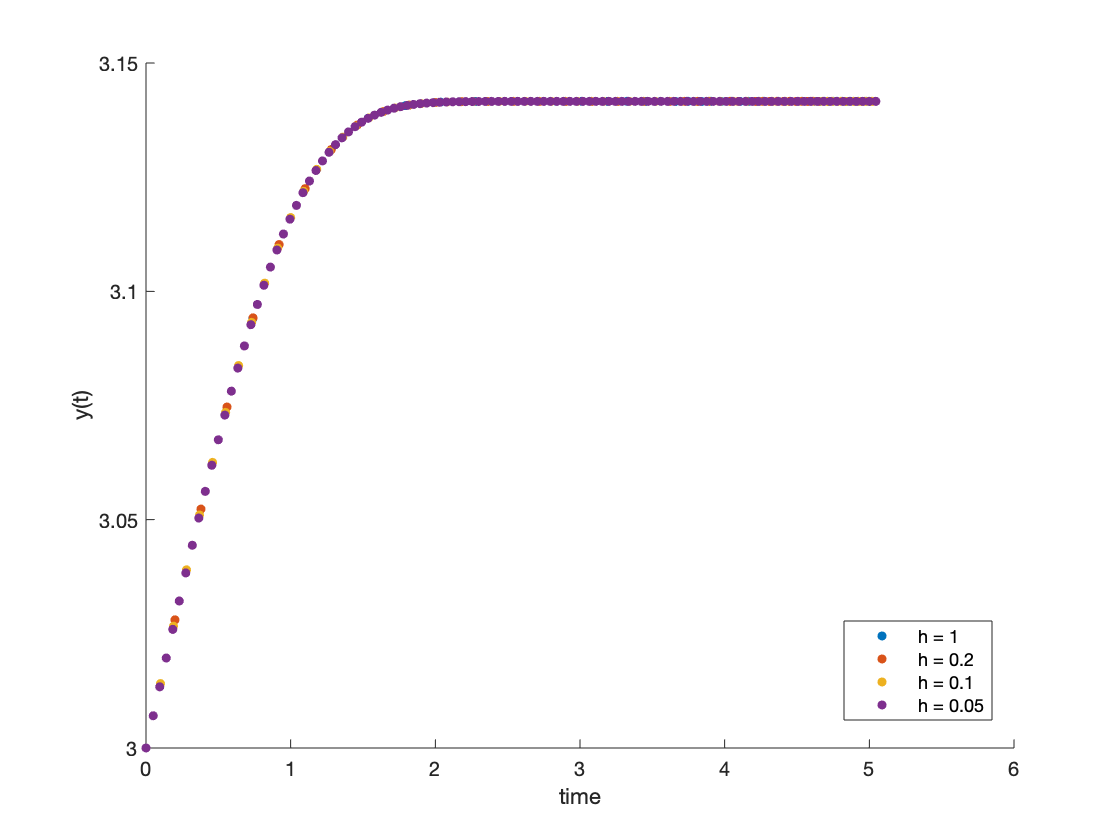
\includegraphics[width=\textwidth]{rk_adapt_t_5.png}
\caption{Runge-Kutta 45 Adaptive Method}
\label{fig:time4}
\end{subfigure}

\caption{Numerical methods; (a) Euler Method, (b) Euler Midpoint Method, (c) Runge-Kutta Method, (d) Runge-Kutta 45 Adaptive Method. All sub figures were plotted using 4 various step sizes from $h = 1$ to $h = 0.05$ and $t = 5$.}
\label{fig:time}

\end{figure}

\newpage

\begin{figure}[htp]
\centering

\begin{subfigure}{0.49\columnwidth}
\centering
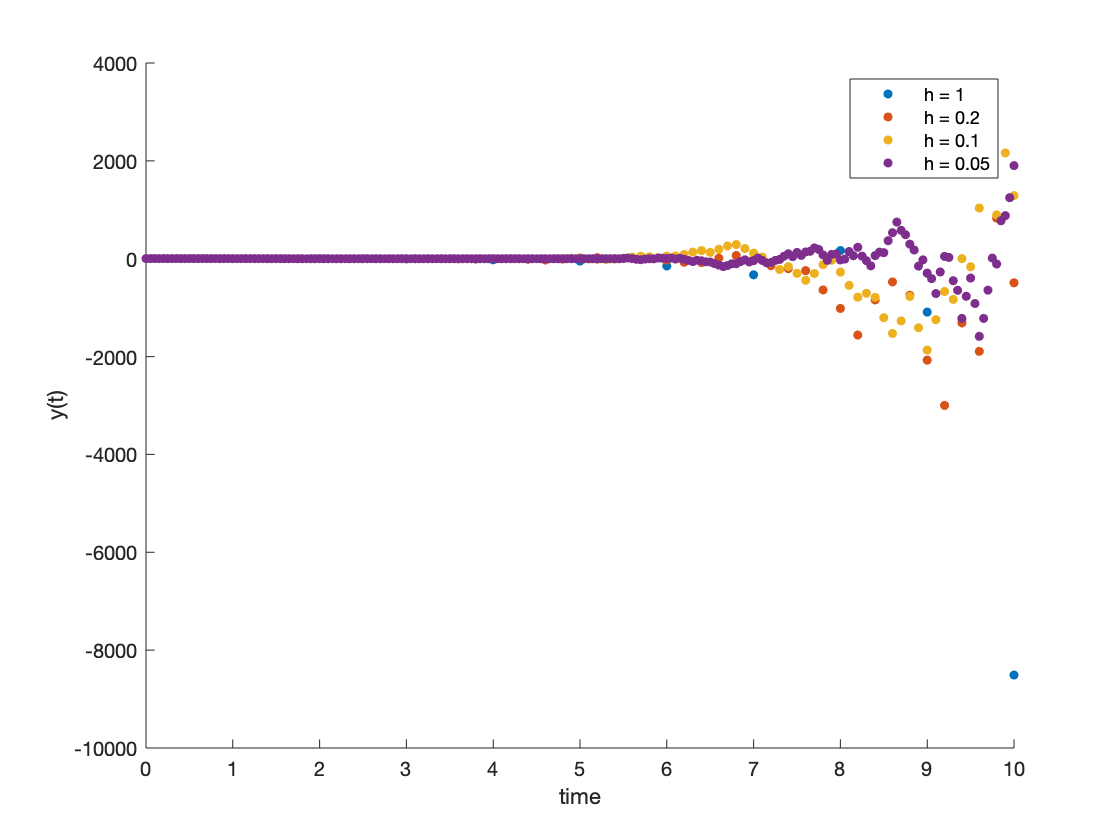
\includegraphics[width=\textwidth]{euler_t_10.png}
\caption{Euler Method}
\label{fig:time1}
\end{subfigure}\hfill
\begin{subfigure}{0.49\columnwidth}
\centering
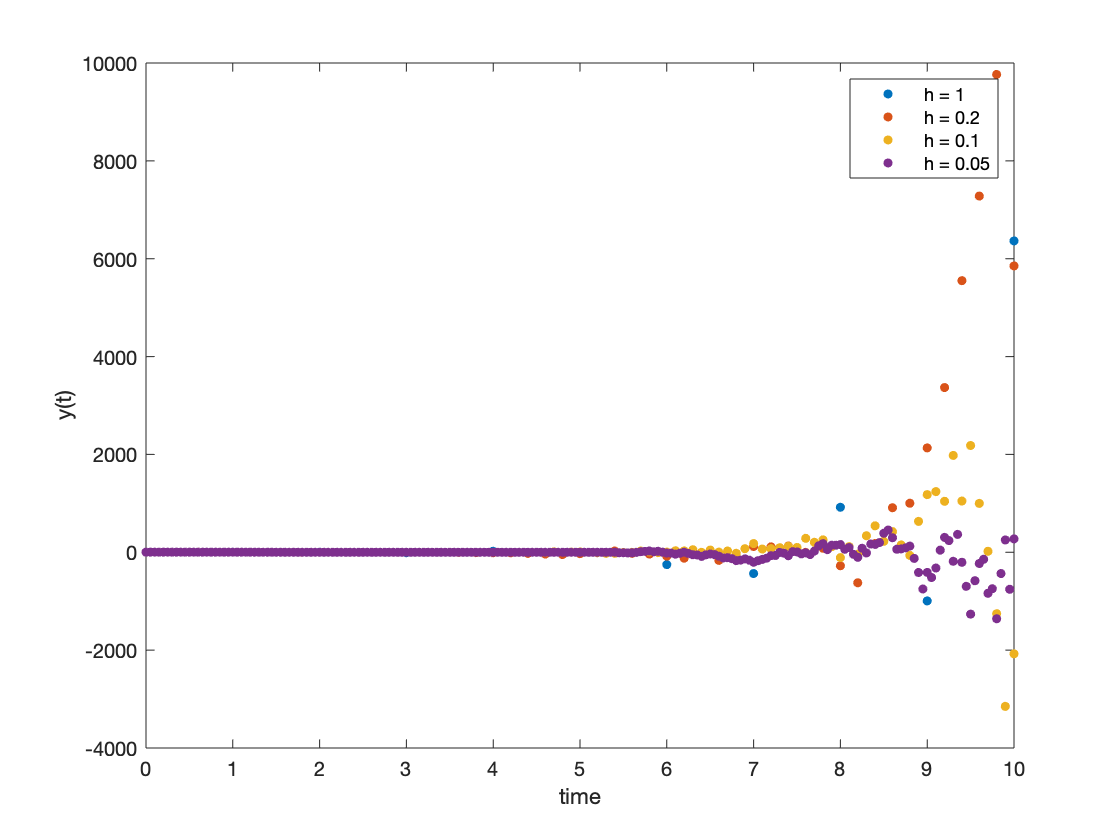
\includegraphics[width=\textwidth]{euler_mid_t_10.png}
\caption{Euler Midpoint Method}
\label{fig:time2}
\end{subfigure}

\medskip

\begin{subfigure}{0.49\columnwidth}
\centering
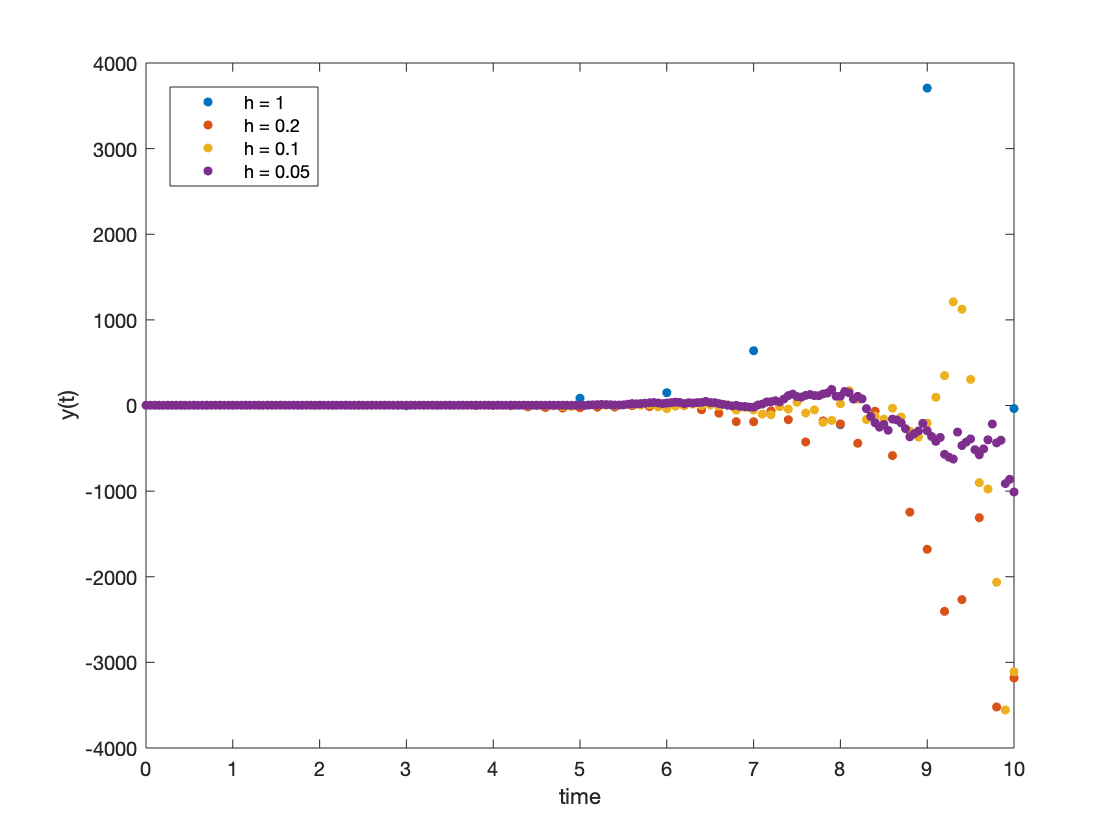
\includegraphics[width=\textwidth]{rk_t_10.png}
\caption{Runge-Kutta Method}
\label{fig:time3}
\end{subfigure}\hfill
\begin{subfigure}{0.49\columnwidth}
\centering
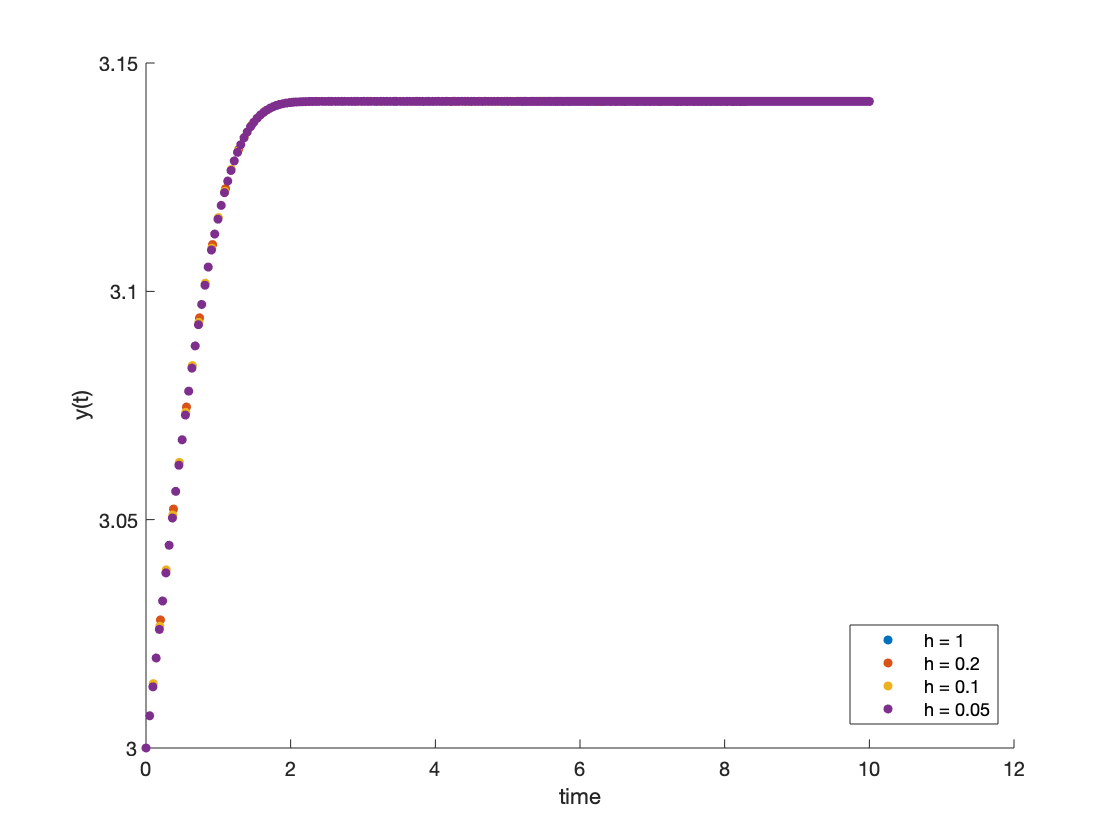
\includegraphics[width=\textwidth]{rk_adapt_t_10.png}
\caption{Runge-Kutta 45 Adaptive Method}
\label{fig:time4}
\end{subfigure}

\caption{Numerical methods; (a) Euler Method, (b) Euler Midpoint Method, (c) Runge-Kutta Method, (d) Runge-Kutta 45 Adaptive Method. All sub figures were plotted using 4 various step sizes from $h = 1$ to $h = 0.05$ and $t = 10$.}
\label{fig:time}

\end{figure}

\newpage

\section*{Problem 2}

Using the Runge-Kutta adaptive method to solve 

$$
\frac{dP}{dt} = mg - kv^{2}
$$

produces Figure 4.

\begin{figure}[h!]
    \centering
    {{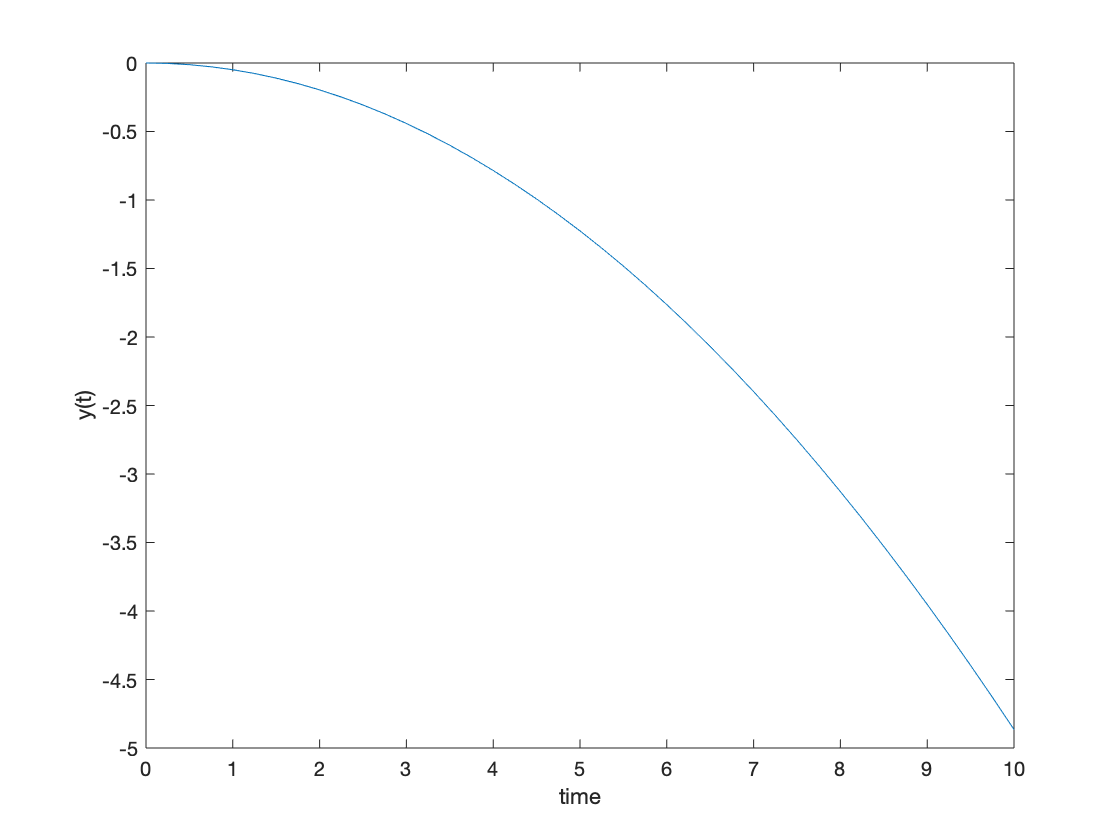
\includegraphics[width=15cm]{problem_2.png}}}%
    \qquad
    \caption{Runge-Kutta method with a negative initial time value.}%
    \label{fig:example}%
\end{figure}

\newpage

\section*{Problem 3}

This problem is not possible to solve. In this problem it is the first time we see an interval that starts with a negative value $-1 \leq x \leq 1$. However, this is not the problem. Having an interval that goes from a negative value to a positive one is possible and this can be proven by running the first problem from the interval $-10 \leq t \leq 10$. The figure below gives an example of negative intervals in problem 1.

\begin{figure}[h!]
    \centering
    {{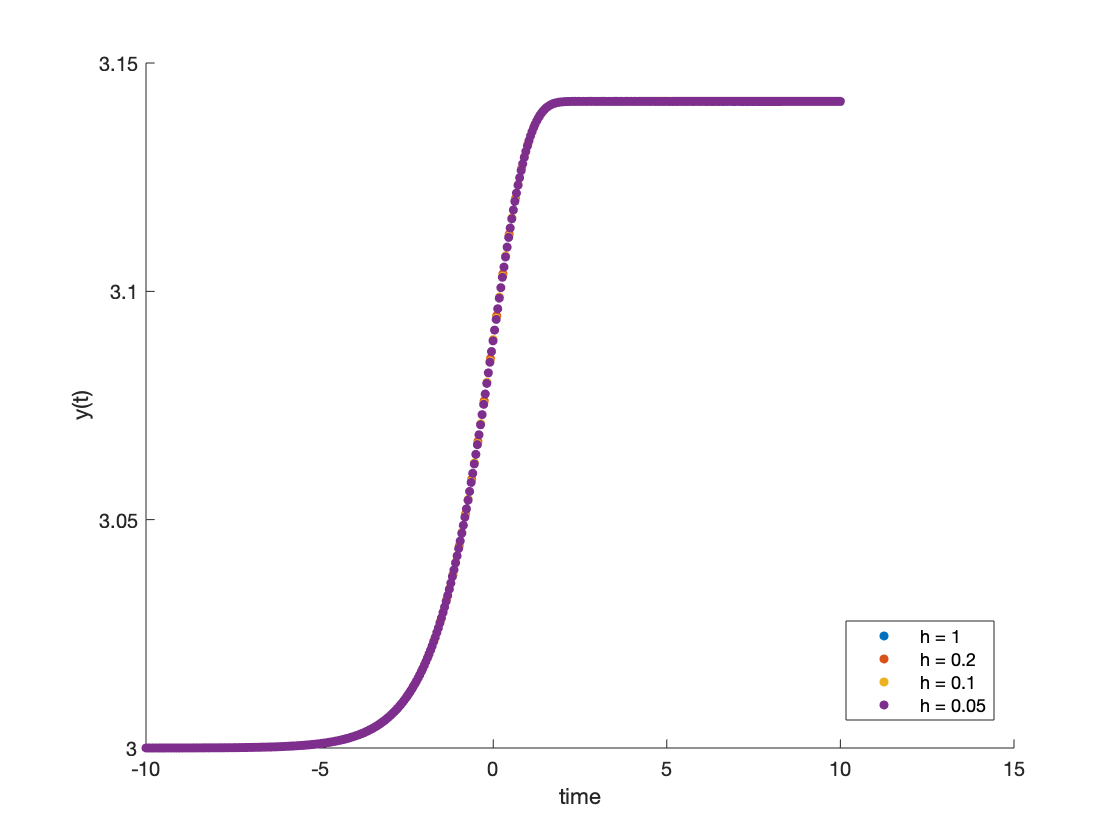
\includegraphics[width=15cm]{rk_neg_t.png}}}%
    \qquad
    \caption{Runge-Kutta method with a negative initial time value.}%
    \label{fig:example}%
\end{figure}

\newpage

The problem lies in the initial value which is gave as 

$$
y(-1) = 1.
$$

Using the same notation this would be programmed in Matlab as $y(0) =  1$. However indexing in matlab starts at 1. Thus, this problem never gives the proper $y_{0}$ value and a solution can not be found.

\newpage

\section*{Problem 4}

To be able to run this system through the Runge-Kutta, the matlab code needs to be edited in such a way that the initial values take in a vector with two elements. Furthermore, the derivative function also has to resemble the same vector. After editing the function, figure 6 is the output we get from the system.

\begin{figure}[h!]
    \centering
    {{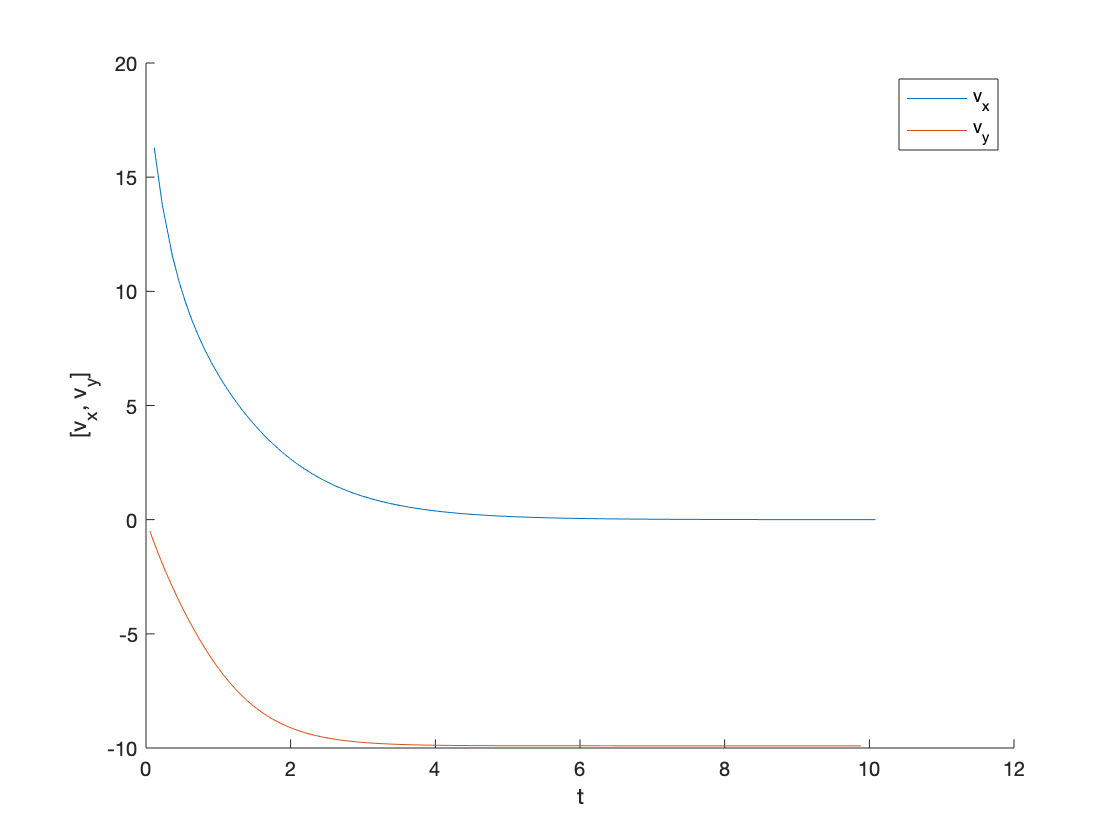
\includegraphics[width=15cm]{problem_4.png}}}%
    \qquad
    \caption{2-D differential equation system.}%
    \label{fig:example}%
\end{figure}

\newpage

\section*{Problem 5}

Much like the previous system this system needs to be edited in the same way.  The matlab code needs to be edited in such a way that the initial values take in a vector with four elements. Furthermore, the derivative function also has to resemble the same vector with four elements. The output from this system is shown in Figure 7.


\begin{figure}[h!]
    \centering
    {{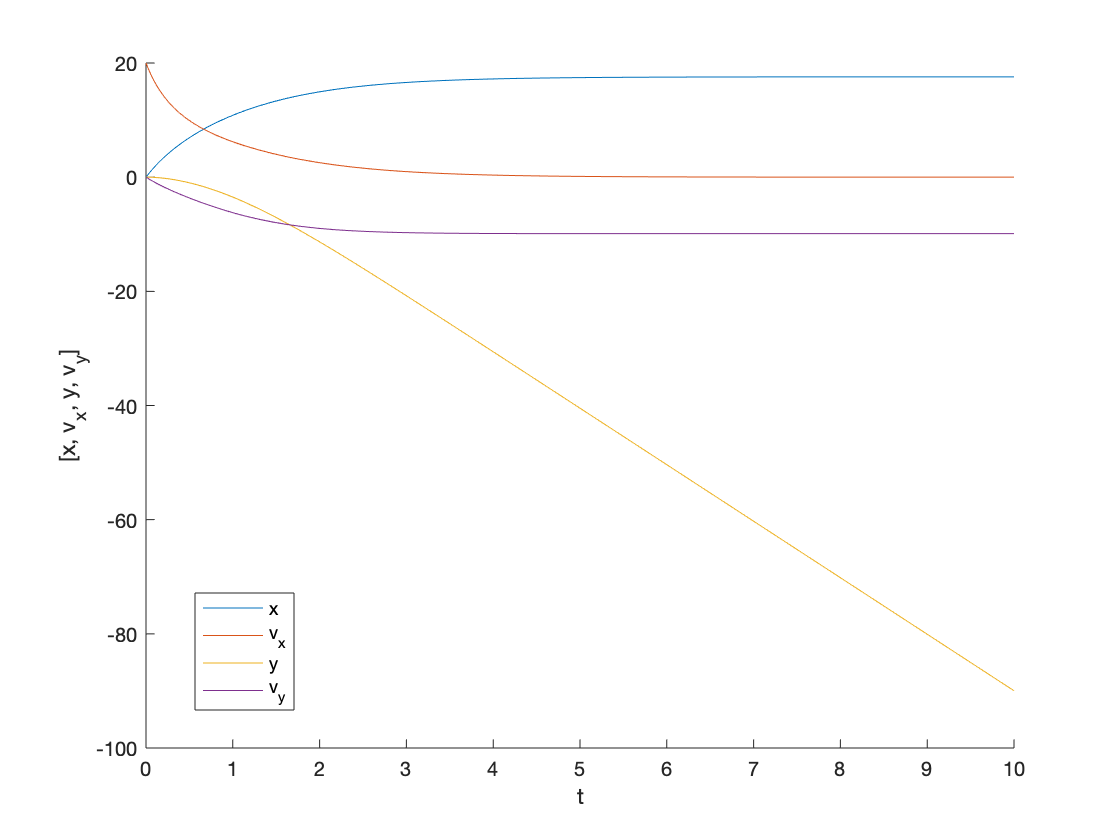
\includegraphics[width=15cm]{problem_5.png}}}%
    \qquad
    \caption{2-D second order differential equation system.}%
    \label{fig:example}%
\end{figure}


% --------------------------------------------------------------
%                           End Document.
% --------------------------------------------------------------
 
\end{document}

